% \subsection{Addressing closed-loop identification bias}\label{sec:CL_ID_issue}
% Correlation between inputs and preceding noise produces a bias for the underlying identification task in \ac{DeePC}~\citep{Dinkla2023}. This section demonstrates this issue for adaptive controller implementations using simulations.
%
% \noindent By means of simulations, this section will show the superior performance of \ac{CL-DeePC} compared to \ac{DeePC}, thereby providing contribution~5. A reference tracking case is first examined. Thereafter, the closed-loop correlation between inputs and noise is visualized. Subsequently, the resulting consistency and inconsistency of respectively \ac{CL-DeePC} and \ac{DeePC} predictors is shown.
% 
\subsection{Example of a reference tracking case}
\noindent To compare the performance of \ac{DeePC} and \ac{CL-DeePC} in an adaptive setting this section presents a reference tracking example by Fig.~\ref{fig:CL_Problem_Solution}. \ac{CL-DeePC} clearly manages considerably better reference tracking performance w.r.t. \ac{DeePC}, the former performing comparably to the oracle. At first, all of the data that the data-driven controllers rely on derives from open-loop operation. Due to the adaptive nature of the controller implementation, after $\bar{N}$ time steps, all of the employed data derives from closed-loop operation. The reference tracking ability of \ac{DeePC} appears to decrease as the amount of employed closed-loop data increases. Thereafter, a cyclical behaviour may be observed for \ac{DeePC}: large reference tracking errors that result from, e.g., the closed-loop identification issue momentarily increase the signal-to-noise ratio and thereby temporarily improve the obtained reference tracking performance again.
% ------------------------- Figure --------------------------
\begin{figure}[b!]
\begin{center}%
\includegraphics[width=\columnwidth]{results/figures/DeePC_CL_ID_issue_Re_1_Nbar_239_p_20_f_20_Ru_1_Rdu_0_Q_100_R_0_dR_10.pdf}    % The printed column  
\caption{Reference tracking by adaptive \ac{DeePC} and \ac{CL-DeePC} using \ac{IVs}. After the vertical line at $\bar{N}$ all used data originates from operation in closed-loop. \ac{CL-DeePC} displays better reference tracking performance than \ac{DeePC}, in part due to a closed-loop identification problem.}% width is 8.4 cm.
\label{fig:CL_Problem_Solution}%                                 % Size the figures 
\end{center}%                                 % accordingly.
\end{figure}%
% -----------------------------------------------------------

\subsubsection{Correlation between inputs and noise}
\noindent This section demonstrates the existence of correlation between inputs and preceding noise during closed-loop operation in an adaptive setting by means of simulations. Following the preceding consistency proof in \secref{sec:Theorem1}, the correlation matrix of interest is given by $E_{i_p,f_\mathrm{ID},N}\begin{bmatrix}U_{i,p,N}^\top & U_{i_p,f_\mathrm{ID},N}^\top\end{bmatrix}$, with $f_\mathrm{ID}=f$ for \ac{DeePC}, and $f_\mathrm{ID}=1$ for \ac{CL-DeePC}. Fig.~\ref{fig:EfUpf_correlation} shows the average of this correlation matrix based on the closed-loop data of 120 different noise realizations. Based on the figure, between \ac{DeePC} and \ac{CL-DeePC}, only \ac{DeePC} experiences the correlation that it induces between inputs and noise. Note that the stochastic variability of subsequent control policies, which arises from the adaptive implementation in the presence of noise, is insufficient to mitigate the input-noise correlation experienced by \ac{DeePC}.
% ------------------------- Figure --------------------------
\begin{figure}[b!]
\begin{center}
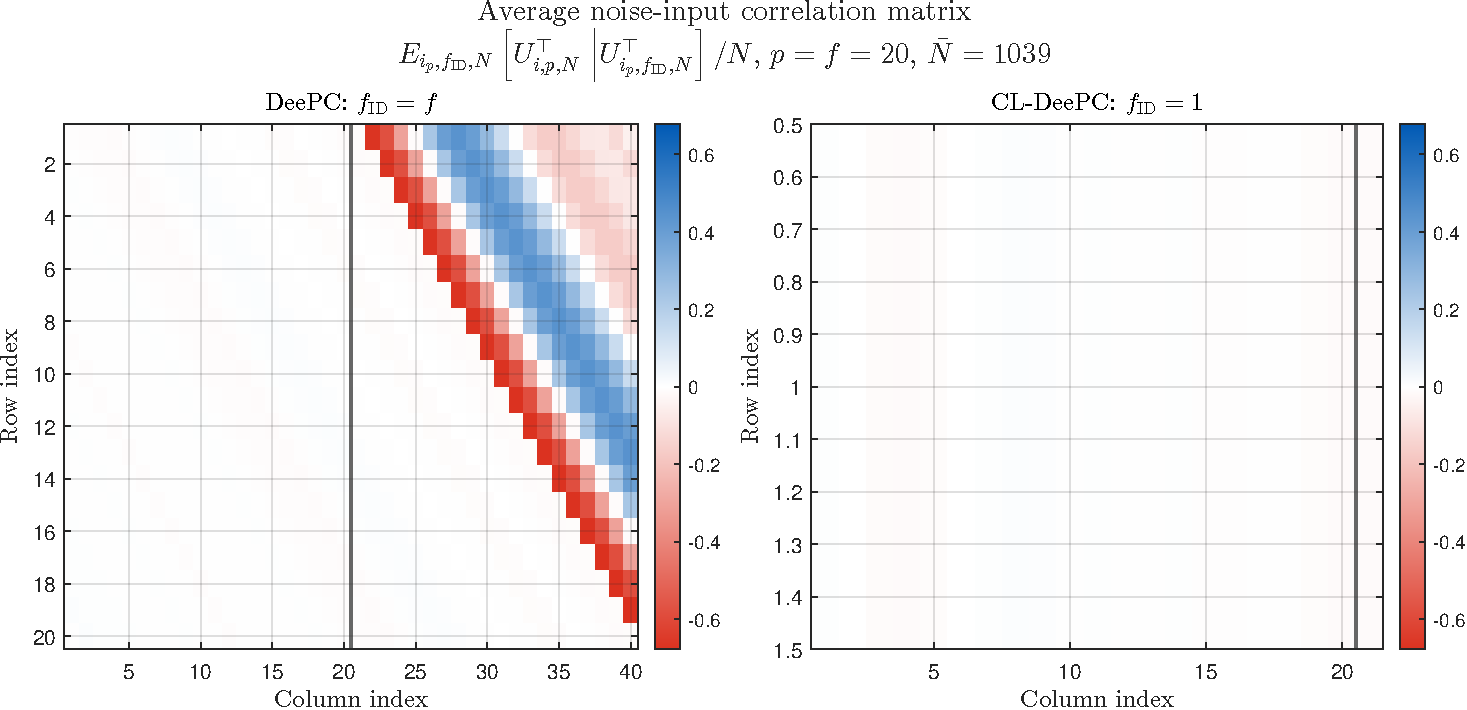
\includegraphics[width=\columnwidth]{results/figures/Correlation_Nbar_1039_p_20_f_20_Re_1_Ru_1_Rdu_0_Q_100_R_0_dR_10.pdf}    % The printed column  
\caption{Noise-input correlation matrix for \ac{DeePC} and \ac{CL-DeePC} averaged over the closed-loop data from 120 noise realizations. In contrast to \ac{DeePC}, \ac{CL-DeePC} makes use of input data that is uncorrelated with preceding noise.}  % width is 8.4 cm.
\label{fig:EfUpf_correlation}                                 % Size the figures 
\end{center}                                 % accordingly.
\end{figure}
% -----------------------------------------------------------

\subsubsection{Consistency analysis}
\noindent This section demonstrates the consistency (or lack thereof) of the estimators employed by \ac{DeePC} and \ac{CL-DeePC} as a result of experienced closed-loop input-noise correlation. Along the lines of the consistency analysis in \secref{sec:Theorem1} and~\cite{Dinkla2023} it is to be expected that the implicit matrix estimate of $\mathcal{T}_{f_\mathrm{ID}}^\mathrm{u}$ is inconsistent for \ac{DeePC} ($f_\mathrm{ID}=f$) and consistent for \ac{CL-DeePC} ($f_\mathrm{ID}=1$). For a fair comparison, the error in $\widehat{\mathcal{T}}_f^\mathrm{u}$ is shown for both controllers by Fig.~\ref{fig:Tuf_consistency}. \secref{sec:Sequential} is followed to construct this estimate for \ac{CL-DeePC}.

As expected, as the number of employed past data points $\bar{N}$ increases (together with the number of columns $N=\bar{N}-p-f_\mathrm{ID}+1$), the bias of the \ac{CL-DeePC} estimate keeps decreasing, which indicates that the employed estimate is indeed consistent. In contrast, for \ac{DeePC} the bias does not keep decreasing noticeably beyond around $\bar{N}=400$, indicating that the implicitly employed estimate $\widehat{\mathcal{T}}_f^\mathrm{u}$ is inconsistent.
% ------------------------- Figure --------------------------
\begin{figure}[b!]
\begin{center}
\includegraphics[width=\columnwidth]{results/figures/Consistency_Nbar_99-1039-50_p_20_f_20_Re_1_Ru_1_Rdu_0_Q_100_R_0_dR_10.pdf}    % The printed column  
\caption{Bias of the implicitly estimated matrix $\mathcal{T}_f^\mathrm{u}$ based exclusively on adaptive closed-loop operation. Shaded regions indicate the 10\textsuperscript{th}, 30\textsuperscript{th}, 70\textsuperscript{th} and 90\textsuperscript{th} percentiles of 120 simulations with different noise realizations.}%Increasingly narrow regions around the median contain 80\% and 40\% of the data.}  % width is 8.4 cm.
\label{fig:Tuf_consistency}                                 % Size the figures 
\end{center}                                 % accordingly.
\end{figure}
% -----------------------------------------------------------